\documentclass{beamer}
\usepackage[utf8]{inputenc}
\usepackage{caption}
\usepackage{subcaption}
\usepackage{amsmath}
\usepackage{tikz}

\title{Math Camp Day 1}
\author{Ben Adenbaum, Juanita Duque-Rosero, Ryan Maguire, Kameron McCombs}
\date{June 2021}
\usenavigationsymbolstemplate{}
\setbeamertemplate{footline}[frame number]
\begin{document}
    \maketitle
    \begin{frame}{Outline}
        Today we'll talk about the following subjects and get a brief
        introduction to each.
        \begin{itemize}
            \item Graphs
            \item Surfaces and Topology
            \item Planarity
            \item Genus
        \end{itemize}
        Don't worry if you've never heard of any of these before, it is not expected of you.
    \end{frame}
    \begin{frame}{Graphs}
        \begin{itemize}
            \item What are graphs?
            \item How were they developed?
            \item How are they used?
            \item What are some simple properties of graphs?
        \end{itemize}
    \end{frame}
    \begin{frame}{Graphs}
        \begin{definition}
            A graph is a set of vertices and a set of edges connecting
            the vertices.
        \end{definition}
        The graph in Fig.~\ref{fig:graph_example_001} has 4 vertices and 3 edges.
        Note that no vertex has an edge connecting back to itself, and no two
        vertices have more than 1 edge between them. When this happens, we say
        the graph is a \textit{simple} graph.
        \begin{figure}
            \centering
            \includegraphics{figs/graph_example_001.eps}
            \caption{An example of a graph}
            \label{fig:graph_example_001}
        \end{figure}
    \end{frame}
    \begin{frame}{Graphs}
        It is possible for a graph to have multiple edges between 2 vertices.
        When this happen, we call the graph a \textit{multigraph}. Multigraphs will
        be important when talking about knot theory, since knots and multigraphs turn
        out to be very similar.
        \par\hfill\par
        Fig.~\ref{fig:multigraph_example_001} shows a multigraph. It is not a simple graph
        there are 2 vertices with 3 edges between them.
        \begin{figure}
            \centering
            \includegraphics{figs/multigraph_example_001.eps}
            \caption{A multigraph}
            \label{fig:multigraph_example_001}
        \end{figure}
    \end{frame}
    \begin{frame}{Graphs}
        One of the simplest features to study in graphs are \textit{paths}.
        A path is obtained by starting at a particular vertex, walking along an
        edge to another vertex, and continuing until you wish to stop. A
        \textit{cycle} is obtained by starting and ending at the same vertex without
        using the same edge more than once.
        \begin{figure}
            \centering
            \includegraphics{figs/graph_example_002.eps}
            \caption{A graph with a cycle}
            \label{fig:graph_example_002}
        \end{figure}
    \end{frame}
    \begin{frame}{Graphs}
        A connected graph is a graph in which there is a path
        between any two vertices. In other words, any two vertices
        can be \textit{connected} by a sequence of edges.
        \begin{figure}
            \centering
            \begin{subfigure}[b]{0.49\textwidth}
                \centering
                \includegraphics{figs/graph_example_connected_001.eps}
                \caption{A connected graph}
                \label{fig:onnected_graph}
            \end{subfigure}
            \begin{subfigure}[b]{0.49\textwidth}
                \centering
                \includegraphics{figs/graph_example_disconnected_001.eps}
                \caption{A disconnected graph}
                \label{fig:disonnected_graph}
            \end{subfigure}
        \end{figure}
    \end{frame}
    \begin{frame}{Graphs}
        \begin{definition}
            A \textit{tree} is a connected graph that has
            zero cycles in it.
        \end{definition}
        The reason for the name is obvious if we look at something called a
        \textit{binary} tree. The graph looks something like an actual tree.
        Fig.~\ref{fig:graph_example_003} shows a binary tree.
        \begin{figure}
            \centering
            \includegraphics{figs/graph_example_003.eps}
            \caption{A binary tree}
            \label{fig:graph_example_003}
        \end{figure}
    \end{frame}
    \begin{frame}{Graphs}
        Unfortunately, not all \textit{trees} need to look like trees.
        The graph in Fig.~\ref{fig:graph_example_004} has no cycles in it,
        and is therefore a tree. However, it does not look like an actual tree.
        \begin{figure}
            \centering
            \includegraphics{figs/graph_example_004.eps}
            \caption{Another tree}
            \label{fig:graph_example_004}
        \end{figure}
    \end{frame}
    \begin{frame}{Graphs}
        The first major problem in graph theory is the \textit{Seven Bridges of K\"{o}nigsberg}.
        The city of K\"{o}nigsberg has seven bridges, and to make travel and delivery costs more efficient,
        the question was asked as to whether or not it is possible to cross all seven bridges once and
        only once. That is, no repeats of bridges are allowed, and no bridges are left out.
        \begin{figure}
            \centering
            \includegraphics{figs/bridges_of_konigsberg_001.eps}
            \caption{The seven bridges of K\"{o}nigsberg}
            \label{fig:bridges_001}
        \end{figure}
    \end{frame}
    \begin{frame}{Graphs}
        It turns out the problem is impossible to solve. In other words, there is no solution.
        The solution came from the mathematician Leonhard Euler who pointed out that the grass and
        the rivers are not important, only the land masses and bridges, which we can label as
        vertices and edges of a graph. The result is Fig.~\ref{fig:bridges_002}.
        \begin{figure}
            \centering
            \includegraphics{figs/bridges_of_konigsberg_002.eps}
            \caption{The seven bridges of K\"{o}nigsberg as a multigraph}
            \label{fig:bridges_002}
        \end{figure}
    \end{frame}
    \begin{frame}{Graphs}
        The solution goes like this.
        \begin{itemize}
            \item With the exception of the start and end vertices,
                every vertex must have an \textit{even} number of edges.
            \item The start and end vertices are the only ones that can have an odd number
                of edges.
            \item There are at most 2 vertices that can have an odd number of edges.
            \item All 4 vertices in the bridges of K\"{o}nigsberg problem have an odd number of edges.
            \item There is no solution.
        \end{itemize}
    \end{frame}
    \begin{frame}{Graphs}
        Because of Euler's solution, the phrase \textit{Eulerian path} refers to a path through
        a graph in which every edge is crossed exactly once. 
        \par\hfill\par
        Here's another graph, called the \textit{Haus vom Nikolaus} graph. Try to find an
        Eulerian path through it.
        \begin{figure}
            \centering
            \includegraphics{figs/haus_vom_nikolaus_puzzle_001.eps}
            \caption{The Haus vom Nikolaus graph}
            \label{fig:haus_001}
        \end{figure}
    \end{frame}
    \begin{frame}{Graphs}
        Since the bottom two vertices have an odd number of edges connected to them,
        and the rest are even, we know an Eulerian path must start at one of these and
        end at the other.
        The graph below is called the \textit{Annie Pope} graph. Does it have an Eulerian path?
        \begin{figure}
            \centering
            \includegraphics{figs/annie_pope_graph_001.eps}
            \caption{The Annie Pope graph}
            \label{fig:annie_001}
        \end{figure}
    \end{frame}
    \begin{frame}{Graphs}
        Before moving on, it might be fun to talk about one of the \textit{famous} problems in
        graph theory. It's not famous amongst mathematicians, but the problem somehow found its
        way to the center of the movie \textit{Good Will Hunting}. It involves
        \textit{irreducible} trees, and trying to find all of them. The movie claims it took
        M.I.T. mathematicians 2 years to solve it, but we can probably figure it out in 15 minutes.
    \end{frame}
    \begin{frame}{Graphs}
        An \textit{irreducible} tree is a tree that has no redundant vertices. A redundant
        vertex is one where there's only one way in and one way out. In other words, a redundant
        vertex has exactly 2 edges attached to it. It's redundant because there's nothing really
        happening at that vertex, and it may as well be treated as part of an edge.
        \begin{figure}
            \centering
            \begin{subfigure}[b]{0.32\textwidth}
                \centering
                \resizebox{\textwidth}{!}{%
                    \includegraphics{figs/reducible_tree_002.eps}
                }
                \caption{A reducible tree}
                \label{fig:reducible_tree_002}
            \end{subfigure}
            \begin{subfigure}[b]{0.32\textwidth}
                \centering
                \resizebox{\textwidth}{!}{%
                    \includegraphics{figs/reducible_tree_001.eps}
                }
                \caption{A \textit{very} reducible tree}
                \label{fig:reducible_tree_001}
            \end{subfigure}
            \begin{subfigure}[b]{0.32\textwidth}
                \centering
                \resizebox{\textwidth}{!}{%
                    \includegraphics{figs/irreducible_tree_001.eps}
                }
                \caption{An irreducible tree}
                \label{fig:irreducible_tree_001}
            \end{subfigure}
        \end{figure}
    \end{frame}
    \begin{frame}{Graphs}
        The problem is to find all 10 irreducible trees with 10 vertices.
    \end{frame}
    \begin{frame}{Graphs}
        Below are all 10.
        \begin{figure}
            \centering
            \resizebox{!}{0.7\textheight}{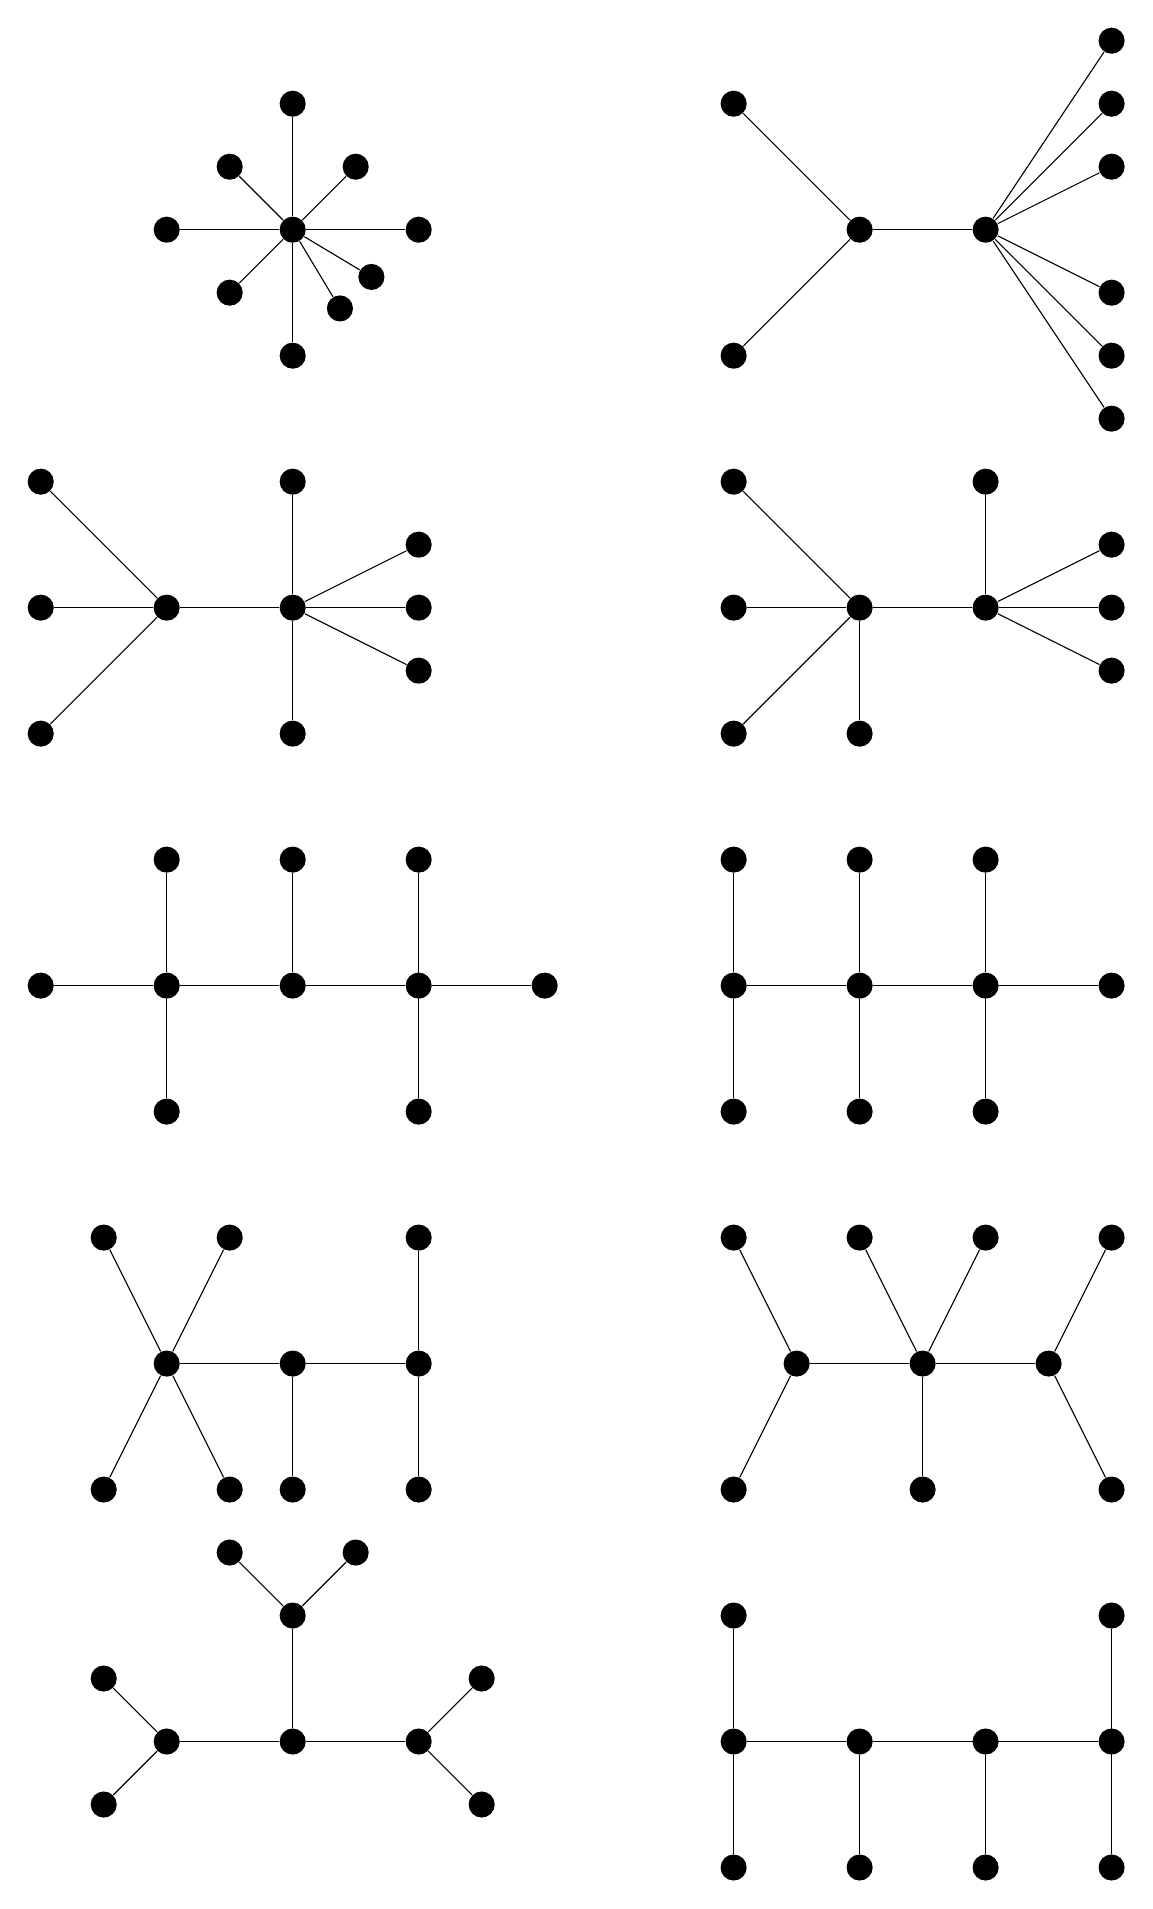
\begin{tikzpicture}[scale = .8]
\node[fill, circle] (A) at (0,0) {}; 
\node[fill, circle] (B) at (2,0) {}; 
\node[fill, circle] (C) at (1,1) {}; 
\node[fill, circle] (D) at (0,2) {}; 
\node[fill, circle] (E) at (-1,1) {}; 
\node[fill, circle] (F) at (-2,0) {}; 
\node[fill, circle] (G) at (-1,-1) {}; 
\node[fill, circle] (H) at (0,-2) {}; 
\node[fill, circle] (I) at (.75,-1.25) {}; 
\node[fill, circle] (J) at (1.25,-.75) {}; 
\draw[-] (A) -- (B);
\draw[-] (A) -- (C);
\draw[-] (A) -- (D);
\draw[-] (A) -- (E);
\draw[-] (A) -- (F);
\draw[-] (A) -- (G);
\draw[-] (A) -- (H);
\draw[-] (A) -- (I);
\draw[-] (A) -- (J);


\begin{scope}[shift={(11,0)}]
\node[fill, circle] (A) at (0,0) {}; 
\node[fill, circle] (B) at (2,3) {}; 
\node[fill, circle] (C) at (2,2) {}; 
\node[fill, circle] (D) at (2,1) {}; 
\node[fill, circle] (E) at (2,-1) {}; 
\node[fill, circle] (F) at (2,-2) {}; 
\node[fill, circle] (G) at (2,-3) {}; 
\node[fill, circle] (H) at (-2,0) {}; 
\node[fill, circle] (I) at (-4,-2) {}; 
\node[fill, circle] (J) at (-4,2) {}; 
\draw[-] (A) -- (B);
\draw[-] (A) -- (C);
\draw[-] (A) -- (D);
\draw[-] (A) -- (E);
\draw[-] (A) -- (F);
\draw[-] (A) -- (G);
\draw[-] (A) -- (H);
\draw[-] (H) -- (I);
\draw[-] (H) -- (J);
\end{scope}
\begin{scope}[shift={(0,-6)}]
\node[fill, circle] (A) at (0,0) {}; 
\node[fill, circle] (B) at (0,2) {}; 
\node[fill, circle] (C) at (2,1) {}; 
\node[fill, circle] (D) at (2,0) {}; 
\node[fill, circle] (E) at (2,-1) {}; 
\node[fill, circle] (F) at (0,-2) {}; 
\node[fill, circle] (G) at (-4,0) {}; 
\node[fill, circle] (H) at (-2,0) {}; 
\node[fill, circle] (I) at (-4,-2) {}; 
\node[fill, circle] (J) at (-4,2) {}; 
\draw[-] (A) -- (B);
\draw[-] (A) -- (C);
\draw[-] (A) -- (D);
\draw[-] (A) -- (E);
\draw[-] (A) -- (F);
\draw[-] (H) -- (G);
\draw[-] (A) -- (H);
\draw[-] (H) -- (I);
\draw[-] (H) -- (J);
\end{scope}
\begin{scope}[shift={(11,-6)}]
\node[fill, circle] (A) at (0,0) {}; 
\node[fill, circle] (B) at (0,2) {}; 
\node[fill, circle] (C) at (2,1) {}; 
\node[fill, circle] (D) at (2,0) {}; 
\node[fill, circle] (E) at (2,-1) {}; 
\node[fill, circle] (F) at (-2,-2) {}; 
\node[fill, circle] (G) at (-4,0) {}; 
\node[fill, circle] (H) at (-2,0) {}; 
\node[fill, circle] (I) at (-4,-2) {}; 
\node[fill, circle] (J) at (-4,2) {}; 
\draw[-] (A) -- (B);
\draw[-] (A) -- (C);
\draw[-] (A) -- (D);
\draw[-] (A) -- (E);
\draw[-] (H) -- (F);
\draw[-] (H) -- (G);
\draw[-] (A) -- (H);
\draw[-] (H) -- (I);
\draw[-] (H) -- (J);
\end{scope}
\begin{scope}[shift={(0,-12)}]
\node[fill, circle] (A) at (0,0) {}; 
\node[fill, circle] (B) at (2,0) {}; 
\node[fill, circle] (C) at (4,0) {}; 
\node[fill, circle] (D) at (-2,0) {}; 
\node[fill, circle] (E) at (-4,0) {}; 
\node[fill, circle] (F) at (-2,-2) {}; 
\node[fill, circle] (G) at (-2,2) {}; 
\node[fill, circle] (H) at (2,2) {}; 
\node[fill, circle] (I) at (2,-2) {}; 
\node[fill, circle] (J) at (0,2) {}; 
\draw[-] (A) -- (B);
\draw[-] (B) -- (C);
\draw[-] (A) -- (D);
\draw[-] (D) -- (E);
\draw[-] (D) -- (F);
\draw[-] (D) -- (G);
\draw[-] (A) -- (J);
\draw[-] (H) -- (I);
\end{scope}
\begin{scope}[shift={(9,-12)}]
\node[fill, circle] (A) at (0,0) {}; 
\node[fill, circle] (B) at (0,2) {}; 
\node[fill, circle] (C) at (0,-2) {}; 
\node[fill, circle] (D) at (-2,0) {}; 
\node[fill, circle] (E) at (-2,-2) {}; 
\node[fill, circle] (F) at (-2,2) {}; 
\node[fill, circle] (G) at (2,0) {}; 
\node[fill, circle] (H) at (2,2) {}; 
\node[fill, circle] (I) at (2,-2) {}; 
\node[fill, circle] (J) at (4,0) {}; 
\draw[-] (A) -- (B);
\draw[-] (A) -- (C);
\draw[-] (A) -- (D);
\draw[-] (D) -- (E);
\draw[-] (D) -- (F);
\draw[-] (A) -- (G);
\draw[-] (G) -- (H);
\draw[-] (G) -- (I);
\draw[-] (G) -- (J);
\end{scope}
\begin{scope}[shift={(0,-18)}]
\node[fill, circle] (A) at (0,0) {}; 
\node[fill, circle] (B) at (2,0) {}; 
\node[fill, circle] (C) at (-2,0) {}; 
\node[fill, circle] (D) at (-1,2) {}; 
\node[fill, circle] (E) at (-1,-2) {}; 
\node[fill, circle] (F) at (-3,2) {}; 
\node[fill, circle] (G) at (-3,-2) {}; 
\node[fill, circle] (H) at (0,-2) {}; 
\node[fill, circle] (I) at (2,-2) {}; 
\node[fill, circle] (J) at (2,2) {}; 
\draw[-] (A) -- (B);
\draw[-] (A) -- (C);
\draw[-] (A) -- (H);
\draw[-] (C) -- (E);
\draw[-] (C) -- (F);
\draw[-] (C) -- (D);
\draw[-] (C) -- (G);
\draw[-] (B) -- (I);
\draw[-] (B) -- (J);
\end{scope}
 \begin{scope}[shift={(10,-18)}]
\node[fill, circle] (A) at (3,2) {}; 
\node[fill, circle] (B) at (1,2) {}; 
\node[fill, circle] (C) at (-3,2) {}; 
\node[fill, circle] (D) at (-1,2) {}; 
\node[fill, circle] (E) at (-2,0) {}; 
\node[fill, circle] (F) at (0,0) {}; 
\node[fill, circle] (G) at (2,0) {}; 
\node[fill, circle] (H) at (3,-2) {}; 
\node[fill, circle] (I) at (0,-2) {}; 
\node[fill, circle] (J) at (-3,-2) {}; 
\draw[-] (A) -- (G);
\draw[-] (B) -- (F);
\draw[-] (C) -- (E);
\draw[-] (D) -- (F);
\draw[-] (E) -- (F);
\draw[-] (F) -- (G);
\draw[-] (H) -- (G);
\draw[-] (F) -- (I);
\draw[-] (E) -- (J);
\end{scope}
 \begin{scope}[shift={(0,-24)}]
\node[fill, circle] (A) at (0,0) {}; 
\node[fill, circle] (B) at (0,2) {}; 
\node[fill, circle] (C) at (-1,3) {}; 
\node[fill, circle] (D) at (1,3) {}; 
\node[fill, circle] (E) at (-2,0) {}; 
\node[fill, circle] (F) at (-3,1) {}; 
\node[fill, circle] (G) at (-3,-1) {}; 
\node[fill, circle] (H) at (2,0) {}; 
\node[fill, circle] (I) at (3,1) {}; 
\node[fill, circle] (J) at (3,-1) {}; 
\draw[-] (A) -- (B);
\draw[-] (B) -- (C);
\draw[-] (B) -- (D);
\draw[-] (A) -- (E);
\draw[-] (E) -- (F);
\draw[-] (E) -- (G);
\draw[-] (A) -- (H);
\draw[-] (H) -- (I);
\draw[-] (H) -- (J);
\end{scope}
 \begin{scope}[shift={(10,-24)}]
\node[fill, circle] (A) at (-3,2) {}; 
\node[fill, circle] (B) at (-3,0) {}; 
\node[fill, circle] (C) at (-3,-2) {}; 
\node[fill, circle] (D) at (-1,0) {}; 
\node[fill, circle] (E) at (-1,-2) {}; 
\node[fill, circle] (F) at (1,0) {}; 
\node[fill, circle] (G) at (1,-2) {}; 
\node[fill, circle] (H) at (3,2) {}; 
\node[fill, circle] (I) at (3,0) {}; 
\node[fill, circle] (J) at (3,-2) {}; 
\draw[-] (A) -- (B);
\draw[-] (B) -- (C);
\draw[-] (B) -- (D);
\draw[-] (D) -- (E);
\draw[-] (D) -- (F);
\draw[-] (F) -- (G);
\draw[-] (D) -- (I);
\draw[-] (H) -- (I);
\draw[-] (H) -- (J);
\end{scope}
\end{tikzpicture}}
            \caption{The Good Will Hunting Problem}
            \label{fig:goodwill}
        \end{figure}
    \end{frame}
    \begin{frame}{Complete Graphs}
        The next class of graphs to talk about are the \textit{complete} graphs. These are
        simple graphs where every possible edge is drawn. Because of this, they get very complex
        quickly. Since the only distinguishing feature of a complete graph is the number of
        vertices, the symbol $K_{n}$ denotes the complete graph with $n$ vertices.
        \begin{figure}
            \centering
            \begin{subfigure}[b]{0.49\textwidth}
                \centering
                \includegraphics{figs/graph_example_005.eps}
                \label{fig:graph_example_005}
            \end{subfigure}
            \begin{subfigure}[b]{0.49\textwidth}
                \centering
                \includegraphics{figs/graph_example_006.eps}
                \label{fig:graph_example_006}
            \end{subfigure}
            \caption{Examples of Complete Graphs}
            \label{fig:complex_complete_graphs_001}
        \end{figure}
    \end{frame}
    \begin{frame}{Complete Graphs}
        Complete graphs are often of interest to computer scientists and
        mathematicians since they represent the extreme graphs.
        That is, they have the most possible number of edges on $n$ vertices.
        Best and worst case scenarios of algorithms are often tested on
        these graphs because of this.
        \begin{figure}
            \centering
            \begin{subfigure}[b]{0.49\textwidth}
                \centering
                \includegraphics{figs/graph_example_007.eps}
                \label{fig:graph_example_007}
            \end{subfigure}
            \begin{subfigure}[b]{0.49\textwidth}
                \centering
                \includegraphics{figs/graph_example_008.eps}
                \label{fig:graph_example_008}
            \end{subfigure}
            \caption{More Examples of Complete Graphs}
            \label{fig:complex_complete_graphs_002}
        \end{figure}
    \end{frame}
    \begin{frame}{Complete Graphs}
        Before talking about large complete graphs, we can talk about the small ones.
        The complete graphs $K_{1}$ and $K_{2}$ are very simple. $K_{1}$ has 1 vertex, and so
        the entire graph is a dot. $K_{2}$ has 2 vertices, and 1 edge between them, so we get
        a line segment. These are shown in Figs.~\subref{fig:K_1} and \subref{fig:K_2}.
        \begin{figure}
            \centering
            \begin{subfigure}[c]{0.49\textwidth}
                \centering
                \includegraphics[scale=0.1]{figs/complete_graph_K1.eps}
                \caption{$K_{1}$}
                \label{fig:K_1}
            \end{subfigure}
            \begin{subfigure}[c]{0.49\textwidth}
                \centering
                \includegraphics{figs/complete_graph_K2.eps}
                \caption{$K_{2}$}
                \label{fig:K_2}
            \end{subfigure}
            \label{fig:complete_graphs_003}
        \end{figure}
    \end{frame}
    \begin{frame}{Complete Graphs}
        The next two complete graphs are $K_{3}$ and $K_{4}$. $K_{3}$ has 3 vertices, with
        every vertex adjoined to every other, giving us a triangle. $K_{4}$ is a square with all
        of the edges connecting, giving us a box with an X through it. This is the first of the
        complete graphs where the drawing has an artificial crossing, the point in the center.
        \begin{figure}
            \centering
            \begin{subfigure}[c]{0.49\textwidth}
                \centering
                \includegraphics{figs/complete_graph_K3.eps}
                \caption{$K_{3}$}
                \label{fig:K_3}
            \end{subfigure}
            \begin{subfigure}[c]{0.49\textwidth}
                \centering
                \includegraphics{figs/complete_graph_K4.eps}
                \caption{$K_{4}$}
                \label{fig:K_4}
            \end{subfigure}
        \end{figure}
    \end{frame}
    \begin{frame}{Try to Draw $K_{4}$ without a crossing}
        This crossing has no meaning and is a result of how we've drawn the graph.
        Is is possible to draw this graph without a crossing? Using only straight lines?
        $K_{5}$ is even worse since there are many artificial crossings. Can we draw $K_{5}$
        without any crossings? Try it! If not what are the minimal number of crossings?
        \begin{figure}
            \centering
            \includegraphics{figs/complete_graph_K5.eps}
            \caption{The complete graph $K_{5}$}
            \label{fig:K_5}
        \end{figure}
    \end{frame}
    \begin{frame}{Solution}
        $K_{4}$ can be drawn without crossings, and it can be drawn
        using only straight lines as well. This is not special to $K_{4}$,
        \textit{every} graph that can be drawn without crossings can also be
        drawn without crossings using only straight lines. This is
        \textit{F\'{a}ry's theorem}.
        \begin{figure}
            \centering
            \begin{subfigure}[b]{0.49\textwidth}
            \centering
                \includegraphics{figs/complete_graph_K4_planar.eps}
                \caption{$K_{4}$ without edge crossings}
                \label{fig:K_4_planar}
            \end{subfigure}
            \begin{subfigure}[b]{0.49\textwidth}
                \centering
                \includegraphics{figs/complete_graph_K4_planar_straight_lines.eps}
                \caption{$K_{4}$ using straight lines}
                \label{fig:K_4_planar_straight}
            \end{subfigure}
        \end{figure}
    \end{frame}
    \begin{frame}{Near-Solution}
        For $K_{5}$ it is impossible. The proof of this is a little involved and
        may go beyond the scope of math camp, but the
        \textit{intuitive} proof goes like this. We start
        with $K_{4}$ drawn using only straight lines. If we add a new vertex on the outside of
        the triangle, then the point inside the triangle can't reach the outside one without a
        crossing. Similarly if we place the new vertex in any of the other faces.
        The best we can do is have one crossing.
        \begin{figure}
            \centering
            \includegraphics{figs/complete_graph_K5_almost_planar.eps}
            \caption{A near solution for $K_{5}$}
            \label{fig:K_5_almost_planar}
        \end{figure}
    \end{frame}
    \begin{frame}{Surfaces}
        Since the $K_{5}$ graph needs only one crossing to be drawn, if we could introduce a
        \textit{hole} into the plane then we could get rid of this crossing by going around the
        hole. First note that graph theory can be done on a \textit{sphere} instead of on a
        piece of paper. This is because the plane is \textit{topologically} the same as
        a sphere with a point removed. The way to do this is via
        \textit{stereographic projection}.
    \end{frame}
    \begin{frame}{Surface}
        Stereographic projection is done by placing an observer at the north pole of a sphere.
        Given a point on the sphere, we then draw a straight line between the observer and
        this point, and then continue this line until it hits the $xy$ plane. This will stretch
        the sphere over the entire plane.
        \begin{figure}
            \centering
            \includegraphics{figs/Sphere_Stereographic_Projection.pdf}
            \caption{Stereographic Projection}
            \label{fig:stereo_proj}
        \end{figure}
    \end{frame}
    \begin{frame}{Surface}
        The \textit{intuitive} way to think about a plane being the same as a sphere that has a
        single point missing is to think of an orange. You stab a single hole into the peel, and
        then distort it and flatten it out until you have a circular disk. This idea is shown
        below.
        \begin{figure}
            \centering
            \includegraphics{figs/Sphere_to_Disk_Homeo.pdf}
            \caption{Morphing a sphere with a hole to a disk}
            \label{fig:sphere_to_disk}
        \end{figure}
    \end{frame}
    \begin{frame}{Surfaces}
        The take away is that graph theory can be done on the \textit{surface} of a sphere, and
        all of the results and definitions are the same. With this in mind, perhaps we can do
        graph theory on \textit{other} surfaces. The simplest surface besides a sphere is a
        \textit{torus}, which is the \textit{1-holed} surface. It is shown below.
        \begin{figure}
            \centering
            \includegraphics{figs/torus.eps}
            \caption{A Torus}
            \label{fig:torus}
        \end{figure}
    \end{frame}
    \begin{frame}{Surfaces}
        There are many ways to think about torii. One way is as a \textit{donut} that is hollow.
        Another common way is as a \textit{circle of circles}. We take a circle $C$ and at every
        point of $C$ we attached another circle $C'$. The result is below.
        \begin{figure}
            \centering
            \includegraphics{figs/Torus_Skeleton_Product_Space.pdf}
            \caption{A Circle of Circles}
            \label{fig:torus_2}
        \end{figure}
    \end{frame}
    \begin{frame}{Surfaces}
        The way that will work best for us is by thinking about a square and glue.
        We take a square and \textit{identify} opposite sides. The result is a torus. Can you
        see why?
        \begin{figure}
            \centering
            \includegraphics{figs/square_representation_of_torus.eps}
            \caption{A Torus as a Square}
            \label{fig:square_rep_of_torus}
        \end{figure}
    \end{frame}
    \begin{frame}{Surfaces}
        No need to worry if you can't, it takes a bit of imagination the first time around.
        Let's draw the process.
        \begin{figure}
            \centering
            \includegraphics{figs/Square_to_Torus.eps}
            \caption{Square to a Torus}
            \label{fig:square_to_torus}
        \end{figure}
    \end{frame}
    \begin{frame}{Surfaces}
        Life on a torus is a bit like life in Pac-Man. When you walk around to one edge, you
        instantly appear on the opposite edge. If you lived on this 2D torus you wouldn't know
        there was an edge there. The jumping process would be seamless.
        \begin{figure}
            \centering
            \includegraphics{figs/square_torus_pacman.eps}
            \caption{Two Dimensional Beings on a Torus}
            \label{fig:torus_pacman}
        \end{figure}
    \end{frame}
    \begin{frame}{Surfaces}
        \begin{figure}
            \centering
            \resizebox{!}{0.75\textheight}{%
                \includegraphics{figs/plane_torus_pacman.eps}
            }
            \caption{Two Dimensional Beings on a Torus}
            \label{fig:torus_plane_pacman}
        \end{figure}
    \end{frame}
    \begin{frame}{Surfaces}
        Try to draw $K_{5}$ without crossings on a torus
    \end{frame}
    \begin{frame}{Surfaces}
        The solution is shown below. Remember, the walls are artificial and there are no
        \textit{cuts} in this figure. On the next page we'll redraw this on the entire plane.
        \begin{figure}
            \centering
            \includegraphics{figs/complete_graph_K5_on_flat_torus.eps}
            \caption{$K_{5}$ on a flat torus}
            \label{fig:K_5_flat_torus}
        \end{figure}
    \end{frame}
    \begin{frame}{Surfaces}
        \begin{figure}
            \centering
            \resizebox{!}{0.75\textheight}{%
                \includegraphics{figs/complete_graph_k5_on_torus_plane_cover.eps}
            }
            \caption{$K_{5}$ on a flat torus}
            \label{fig:K_5_flat_torus_plane}
        \end{figure}
    \end{frame}
    \begin{frame}{Solution}
        Of course, the easiest way to visualize this is to draw the lines on a donut.
        \begin{figure}
            \centering
            \includegraphics{figs/complete_graph_K5_on_torus.eps}
            \caption{$K_{5}$ on a torus}
            \label{fig:K_5_torus}
        \end{figure}
    \end{frame}
    \begin{frame}{Solution}
        But what's really nice is that we can use the idea of wrapping the square into a torus
        to get explicit formulae that we can then tell a computer to use and make a 3D picture.
        \begin{figure}
            \centering
            \includegraphics{figs/complete_graph_k5_on_torus_3d.eps}
            \caption{$K_{5}$ on a torus}
            \label{fig:k5_on_3d_torus}
        \end{figure}
    \end{frame}
    \begin{frame}{Utility Problem}
        The next set of graphs to talk about are the \textit{complete bipartite graphs}. It is often best to
        introduce these with a practical problem. A utility company provides water, electricity, and gas to a town.
        Since digging tunnels can be expensive, they want to connect the three utilities to three different houses.
        It would be dangerous to have these utility lines cross, so the question is
        \textit{can we connect the utilities without lines crossing}?
        \begin{figure}
            \centering
            \includegraphics[scale=0.6]{figs/utilities_problem.eps}
            \caption{The Utility Problem}
            \label{fig:utility_problem}
        \end{figure}
    \end{frame}
    \begin{frame}{Utility Problem}
        It turns out, just like $K_{5}$ that this problem is impossible. Below is a \textit{near} solution
        involving only one crossing.
        \begin{figure}
            \centering
            \includegraphics[scale=0.6]{figs/utilities_problem_almost_solution.eps}
            \caption{A Near-Solution the the utility problem}
            \label{fig:utility_problem_almost_solution}
        \end{figure}
    \end{frame}
    \begin{frame}{Bipartite Graphs}
        The utility problem involves something called a
        \textit{bipartite graph}. This is a graph we take
        two rows of vertices and are only allowed to draw an
        edge from the first row to the second row. None of the
        vertices in the first row can have edges between them,
        and similarly none of the edges in the second row.
        \begin{figure}
            \centering
            \begin{subfigure}[b]{0.49\textwidth}
                \centering
                \includegraphics{figs/bipartite_graph_k1_1.eps}
                \caption{$K_{1,1}$}
                \label{fig:bipartite_graph_k1_1}
            \end{subfigure}
            \hfill
            \begin{subfigure}[b]{0.49\textwidth}
                \centering
                \includegraphics{figs/bipartite_graph_k1_2.eps}
                \caption{$K_{1,2}$}
                \label{fig:bipartite_graph_k1_2}
            \end{subfigure}
        \end{figure}
    \end{frame}
    \begin{frame}{Bipartite Graphs}
        A \textit{complete} bipartite graph is one where every
        vertex in the first row is connected to every vertex in
        the second row. Since the only distinguishing feature is the
        number of vertices in the two rows, complete bipartite graphs
        are denoted $K_{m,n}$ where $m$ and $n$ are the number of
        vertices in the first and second rows, respectively.
        \begin{figure}
            \centering
            \begin{subfigure}[b]{0.49\textwidth}
                \centering
                \includegraphics{figs/bipartite_graph_k2_2.eps}
                \caption{$K_{2,2}$}
                \label{fig:bipartite_graph_k2_2}
            \end{subfigure}
            \hfill
            \begin{subfigure}[b]{0.49\textwidth}
                \centering
                \includegraphics{figs/bipartite_graph_k2_2_planar.eps}
                \caption{$K_{2,2}$}
                \label{fig:bipartite_graph_k2_2_planar}
            \end{subfigure}
        \end{figure}
    \end{frame}
    \begin{frame}{Bipartite Graphs}
        The three previous drawings show that $K_{1,1}$ up to
        $K_{2,2}$ can be drawn in the plane without crossings.
        This property has a name.
        \begin{definition}
            A \textit{planar} graph is a graph that can be drawn in the
            plane without crossings.
        \end{definition}
        We've seen that $K_{5}$ is \textit{non-planar}. Below is $K_{3,3}$ which
        is the graph version of the utility problem. It too is \textit{non-planar}.
        \begin{figure}
            \centering
            \includegraphics{figs/bipartite_graph_k3_3.eps}
            \caption{$K_{3,3}$}
            \label{fig:bipartite_graph_k_3_3}
        \end{figure}
    \end{frame}
    \begin{frame}{Bipartite Graphs}
        Rearranging $K_{3,3}$, we see that we can draw it with only 1 crossing,
        all while using straight lines. It is impossible to draw it with zero
        crossings.
        \begin{figure}
            \centering
            \includegraphics{figs/bipartite_graph_k3_3_almost_planar.eps}
            \caption{$K_{3,3}$}
            \label{fig:bipartite_graph_k_3_3_almost_planar}
        \end{figure}
    \end{frame}
    \begin{frame}{Bipartite Graphs}
        If we adopt the arrangement of $K_{3,3}$ from the previous slide, we can get a
        near solution to the utility problem with straight lines.
        \begin{figure}
            \centering
            \includegraphics{figs/utilities_problem_almost_planar.eps}
            \caption{$K_{3,3}$}
            \label{fig:utility_problem_near_planar}
        \end{figure}
    \end{frame}
    \begin{frame}{Bipartite Graphs}
        We saw previously that $K_{5}$ can be drawn without crossings on a torus.
        It turns out $K_{3,3}$ can as well, shown below. Remember, there are no
        cuts in the drawing since this represents a torus.
        \begin{figure}
            \centering
            \includegraphics{figs/bipartite_graph_k3_3_on_flat_torus.eps}
            \caption{$K_{3,3}$ on a torus}
            \label{fig:bipartite_graph_k3_3_on_flat_torus}
        \end{figure}
    \end{frame}
    \begin{frame}{Bipartite Graphs}
        \begin{figure}
            \centering
            \resizebox{!}{0.75\textheight}{%
                \includegraphics{figs/bipartite_graph_k3_3_on_torus_plane_cover.eps}
            }
            \caption{$K_{3,3}$ on a torus}
            \label{fig:K3_3_torus_plane}
        \end{figure}
    \end{frame}
    \begin{frame}{Bipartite Graphs}
        Like the $K_{5}$ drawing, it is easiest to visualize this if we draw it on a donut.
        \begin{figure}
            \centering
            \includegraphics{figs/bipartite_graph_k3_3_on_torus.eps}
            \caption{$K_{3,3}$ on a torus}
            \label{fig:bipartite_graph_k3_3_on_torus}
        \end{figure}
    \end{frame}
    \begin{frame}{Bipartite Graphs}
        Also like $K_{5}$, we can use these notions of gluing the square to get explicit
        formulae we can then tell a computer to use and obtain a 3D image. Below is
        a drawing of $K_{3,3}$ on an actual torus.
        \begin{figure}
            \centering
            \includegraphics{figs/bipartite_graph_k3_3_on_torus_3d.eps}
            \caption{$K_{3,3}$ on a torus}
            \label{fig:bipartite_graph_k3_3_on_torus_3d}
        \end{figure}
    \end{frame}
    \begin{frame}{More Surfaces}
        There are other surfaces we can use besides than the sphere and torus.
        The simplest one after the torus is the \textit{2-holed surface}, also called
        the \textit{genus 2 surface} (we'll see why later). It is shown below.
        \begin{figure}
            \centering
            \includegraphics{figs/two_genus_surface.eps}
            \caption{Two Genus Surface}
            \label{fig:two_genus_surface}
        \end{figure}
    \end{frame}
    \begin{frame}{More Surfaces}
        Just like the genus 1 surface (a torus) can be represented by a square,
        a genus two surface can be represented by an octagon. Below is how we do this.
        \begin{figure}
            \centering
            \includegraphics{figs/octagon_rep_of_two_genus_surface.eps}
            \caption{Two Genus Surface as an Octagon}
            \label{fig:two_genus_surface_octagon_rep}
        \end{figure}
    \end{frame}
    \begin{frame}{More Surface}
        Like the torus and the square, it can be hard to see why this is
        a genus two surface. Let's draw it out.
        \begin{figure}
            \centering
            \includegraphics{figs/octagon_to_2_genus.eps}
            \caption{Two Genus Surface as an Octagon}
            \label{fig:two_genus_surface_octagon}
        \end{figure}
    \end{frame}
    \begin{frame}{More Surfaces}
        One might ask if it's possible to draw $K_{6}$ on a torus without
        crossings, or $K_{7}$. The answer is yes for both (try it on your own later!),
        but $K_{8}$ can not be drawn on a torus without a crossing. It can be drawn on a
        two genus surface without a crossing. The question arises as to whether or not we
        can \textit{always} draw a graph on some surface. First, we give a definition.
        \begin{definition}
            The \textit{genus} of a surface is the number of holes in it.
        \end{definition}
        So, for example, the sphere is a genus 0 surface, the torus is a genus 1 surface, and
        the genus 2 surface is a... genus 2 surface.
    \end{frame}
    \begin{frame}{More Surfaces}
        \begin{theorem}
            It is always possible to draw any graph without crossings
            on some surface of a high enough genus.
        \end{theorem}
        The proof is actually pretty straight forward. First, we start with any graph
        drawn in the plane in any way you'd like. Let's start with the graph below.
        \begin{figure}
            \centering
            \includegraphics{figs/graph_has_genus_001.eps}
            \caption{A Graph}
            \label{fig:graph_has_genus_001}
        \end{figure}
    \end{frame}
    \begin{frame}{More Surfaces}
        At every crossing, attach an object that looks like the \textit{handle} of
        a coffee cup. Because of this resemblance such objects are called
        \textit{handlebodies}. We can now draw lines over and under these handlebodies,
        meaning there are no more crossings.
        \begin{figure}
            \centering
            \includegraphics{figs/graph_has_genus_002.eps}
            \caption{The same without crossings}
            \label{fig:graph_has_genus_002}
        \end{figure}
    \end{frame}
    \begin{frame}{More Surfaces}
        Since graph theory can be done on a sphere, instead of a plane,
        we can also just attached 3 handlebodies to a sphere. The result is
        \textit{topologically} the same as a genus 3 surface.
        \begin{figure}
            \centering
            \begin{subfigure}[c]{0.49\textwidth}
                \includegraphics{figs/three_handlebodies_on_sphere.eps}
                \label{fig:sphere_three_handlebodies}
            \end{subfigure}
            \begin{subfigure}[c]{0.49\textwidth}
                \resizebox{\textwidth}{!}{%
                    \includegraphics{figs/genus_three_surface.eps}
                }
                \label{fig:genus_3_surface}
            \end{subfigure}
            \caption{Different depictions of a genus 3 surface}
        \end{figure}
    \end{frame}
    \begin{frame}{More Surfaces}
        Unfortunately, this algorithm does not give us the
        \textit{smallest} number of handlebodies we need to attach in
        order to draw our graph without crossings. The graph from the
        example is actually planar! We need zero handlebodies!
        The example is the complete bipartite graph $K_{2,3}$ and a planar
        drawing is shown below.
        \begin{figure}
            \centering
            \includegraphics{figs/graph_has_genus_003.eps}
            \caption{$K_{2,3}$}
            \label{fig:K_2_3}
        \end{figure}
    \end{frame}
    \begin{frame}{More Surfaces}
        \begin{definition}
            The \textit{genus} of a graph is the smallest genus of a
            surface needed to draw the graph without crossings.
        \end{definition}
        With this definition, a \textit{planar} graph is simply a genus 0 graph
        since it's a graph that can be drawn on a sphere (or on a plane). We have seen
        that $K_{5}$ and $K_{3,3}$ are genus 1 since they cannot be drawn on the plane,
        but can be drawn on a torus. The question now is the following:
        \textit{are there other surfaces we can draw knots on?}
    \end{frame}
    \begin{frame}{More Surfaces}
        The answer is yes, but these surfaces are very strange. We'll end the day trying to
        describe one of these surfaces, the \textit{Klein bottle}. We start with a
        \textit{M\"{o}bius band}. We made a torus by taking a square, connecting to sides
        into a cylinder, and then attaching the two resulting circles. The Klein bottle is
        constructed in the same way, but with a \textit{twist}. If we take our square and attach
        two of the opposite sides, but with a single twist, we get a M\"{o}bius band.
        \begin{figure}
            \centering
            \includegraphics{figs/Square_to_Mobius_Strip.eps}
            \caption{Creating a M\"{o}bius band}
            \label{fig:square_to_mobius}
        \end{figure}
    \end{frame}
    \begin{frame}{More Surfaces}
        Now we can use this description to draw a M\"{o}bius band.
        Just like a cylinder has a \textit{boundary} (the top and bottom of the cylinder),
        so does a M\"{o}bius band. Unlike the cylinder, which has two boundary parts,
        the M\"{o}bius band has 1, a single closed curve.
        \begin{figure}
            \centering
            \includegraphics{figs/Mobius_Strip.eps}
            \caption{A M\"{o}bius band}
            \label{fig:mobius}
        \end{figure}
    \end{frame}
    \begin{frame}{More Surfaces}
        We're now in a position to describe the Klein bottle.
        Contrast the square below with the one for the torus. Here,
        the $a$ arrows are going in the opposite direction. If we tried
        to perform the same trick with the torus, making a cylinder and then
        connecting the circles, the arrows on the circles wouldn't line up.
        \begin{figure}
            \centering
            \includegraphics{figs/Square_to_Klein_Bottle.eps}
            \caption{Square Representation of a Klein Bottle}
            \label{fig:square_klein}
        \end{figure}
    \end{frame}
    \begin{frame}{More Surface}
        To make them line up requires the surface to \textit{pass through itself}.
        The result is shown below, as well as a transparent version to help visualize.
        \begin{figure}
            \centering
            \begin{subfigure}[b]{0.49\textwidth}
                \centering
                \includegraphics{figs/Klein_Bottle.eps}
                \caption{A Klein Bottle}
                \label{fig:klein}
            \end{subfigure}
            \begin{subfigure}[b]{0.49\textwidth}
                \centering
                \includegraphics{figs/klein_bottle_transparent.eps}
                \caption{A Transparent Klein Bottle}
                \label{fig:klein_transparent}
            \end{subfigure}
        \end{figure}
    \end{frame}
    \begin{frame}{More Surfaces}
        If Pac-Man lived on this surfaced, he may be a bit confused.
        \begin{figure}
            \centering
            \includegraphics{figs/square_klein_bottle_pacman.eps}
            \caption{Pac-Man on a Klein Bottle}
            \label{fig:square_klein_pacman}
        \end{figure}
    \end{frame}
    \begin{frame}{More Surfaces}
        He's not cut in half, but he is able to see both his front and back.
        \begin{figure}
            \centering
            \includegraphics[scale=0.35]{figs/plane_klein_bottle_pacman.eps}
            \caption{Pac-Man on a Klein Bottle}
            \label{fig:square_klein_pacman_plane}
        \end{figure}
    \end{frame}
    \begin{frame}{More Surfaces}
        Like the torus, we can draw $K_{5}$ on a Klein bottle without crossings.
        \begin{figure}
            \centering
            \includegraphics{figs/complete_graph_k5_on_klein_bottle.eps}
            \caption{$K_{5}$ on a Klein Bottle}
            \label{fig:K5_Klein_Bottle}
        \end{figure}
    \end{frame}
    \begin{frame}{Tomorrow}
        Tomorrow we'll talk about:
        \begin{itemize}
            \item Surfaces made from 2, 3, and 4 twists.
            \item Cutting cylinders and M\"{o}bius bands, and these new surfaces.
            \item Knots, classical and \textit{virtual}.
            \item Reidemeister moves for knots.
        \end{itemize}
    \end{frame}
\end{document}
